\documentclass[11pt,border=5pt]{standalone}
\usepackage{fontspec}
\setmainfont{cmunrm.otf}[BoldFont=cmunbx.otf,ItalicFont=cmunti.otf,BoldItalicFont=cmunbi.otf]
\usepackage{amsmath}
\usepackage{unicode-math}
\setmathfont{NewCMMath-Regular.otf}
\usepackage{tikz}
\usetikzlibrary{arrows.meta,patterns,angles,quotes}
\begin{document}
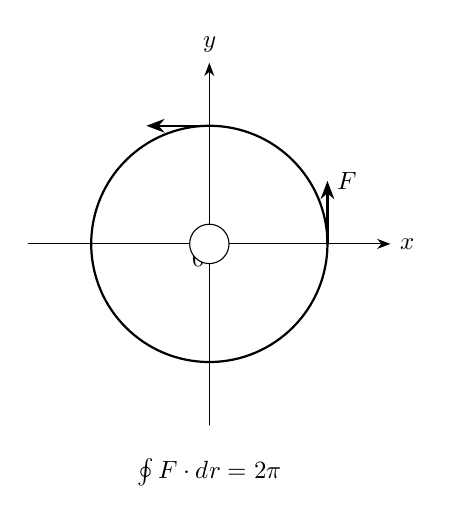
\begin{tikzpicture}[>=Stealth,font=\small,line cap=round,line join=round]
\draw[->,thin] (-2.3,0) -- (2.3,0) node[right] {$x$};
\draw[->,thin] (0,-2.3) -- (0,2.3) node[above] {$y$};
\node at (-0.14,-0.18) {$0$};
\draw[thick] (0,0) circle(1.5);\draw[fill=white] (0,0) circle(.25);\draw[->,thick] (1.5,0) -- (1.5,0.8) node[right] {$F$};
\draw[->,thick] (0,1.5) -- (-0.8,1.5);
\node at (0,-2.9) {$\oint F\cdot dr=2\pi$};

\end{tikzpicture}
\end{document}
